The LHC provides high-luminosity proton-proton collisions with a maximum bunch crossing rate of 40 MHZ, corresponding to 40 TB/s of data.
Due to the limit of buffer size and disk storage, it is impossible to store such amount of data using prsent day technology.
Trigger system are therefore implemented to filter out uninterested events in all the detector readouts, ultimately reducing the event rate to 1 kHz. 
These events are then sent to the CERN tier system for reconstruction and calibration.

\subsection{Level 1 trigger}
A mostly hardware based system called the level 1 trigger system (L1T) is a combination of local and global components (Fig.~\ref{fig:cms_l1t}.
The local trigger systems uses information from a single subdetector, and looks for local patterns such as energy deposit packets, hit patterns, and so on.
The global muon and calorimeter triggers, on the other hand, takes information from corresponding subdetectors and makes very basic reconstruction of physics objects, such as muons, jets, and missing transverse energy to determine whether an event is worth keeping.
The global trigger system then combine information from the local trigger system, and further determines whether an event satisfies the designated requirement.
Once an event meets the requirement of at least one seed, a group of a few criteria, the complete detector information of that event is stored in the front-end buffers and sent to the high level trigger system with a maximal event rate of 100  kHz.

\begin{figure}\centering
    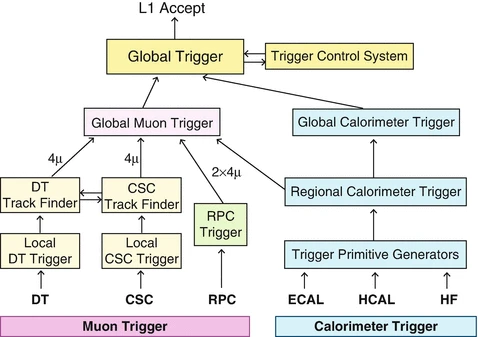
\includegraphics[width=0.85\textwidth]{figure/cms_l1t.png}
    \caption{Architecture of CMS L1 trigger system.}
    \label{fig:cms_l1t}
\end{figure}

\subsection{High level trigger}
In contrast to L1T, The high level trigger (HLT) is entirely software based, and has access to the entire readout data store in the buffer.
Complex calculations, such as offline reconstruction with filter modules and simple object quality sorting are thus allowed in the software.
Physical quantities like shower shape, isolation and track-vertex can be considered as criteria in the menu.
The data sorting can also take advantage of HLT for quick identification of interesting events, such as the SingleMuon data requiring at least 1 muon HLT o be fired.
The HLT provides higher performancce to identify the interested events and further reduce the event rate from 100 kHz to 1 kHz.

To reduce the amount of common (high cross section) events, such as the production of low energy particles, triggers sometimes record just 1 out of $N$ collisions.
The trigger is said to be prescaled by $N$ with such trigger configuration called prescaling.
The number of events recorded by the detector might be enough for common analysis, however, for searches of rare events, prescaling might decrease the integrated luminosity significantly.
